\section{Руководство пользователя}

\subsection{Назначение программы}

Разработанная программа реализует алгоритм сжатия изображений, повторяющий основные этапы стандарта JPEG. 
В отличие от оригинального алгоритма, на этапе энтропийного кодирования используется метод RLE (Run-Length Encoding) 
вместо кодирования по Хаффману. 
Это позволяет упростить реализацию, сохранив при этом все основные свойства алгоритма JPEG.

Программа предназначена для демонстрации полного цикла кодирования и декодирования изображения:

\begin{itemize}
    \item переход от $\textbf{RGB}$ к $\textbf{YCbCr}$
    \item разбиение на блоки $8 \times 8$
    \item дискретное косинус-преобразование (DCT)
    \item квантование
    \item последовательное сканирование (зигзаг)
    \item кодирование RLE
    \item обратные преобразования (IDCT и т. д.)
    \item восстановление RGB-изображения

\end{itemize}



\clearpage
%%%%%%%%%%%%%%%%%%%%%%%%%%%%%%%%%%%%%%%%%%%%%%%%
\subsection{Интерфейс программы}

На рисунке ~\ref{fig:interface} представлено главное окно приложения.

\begin{figure}[h!]
    \centering
    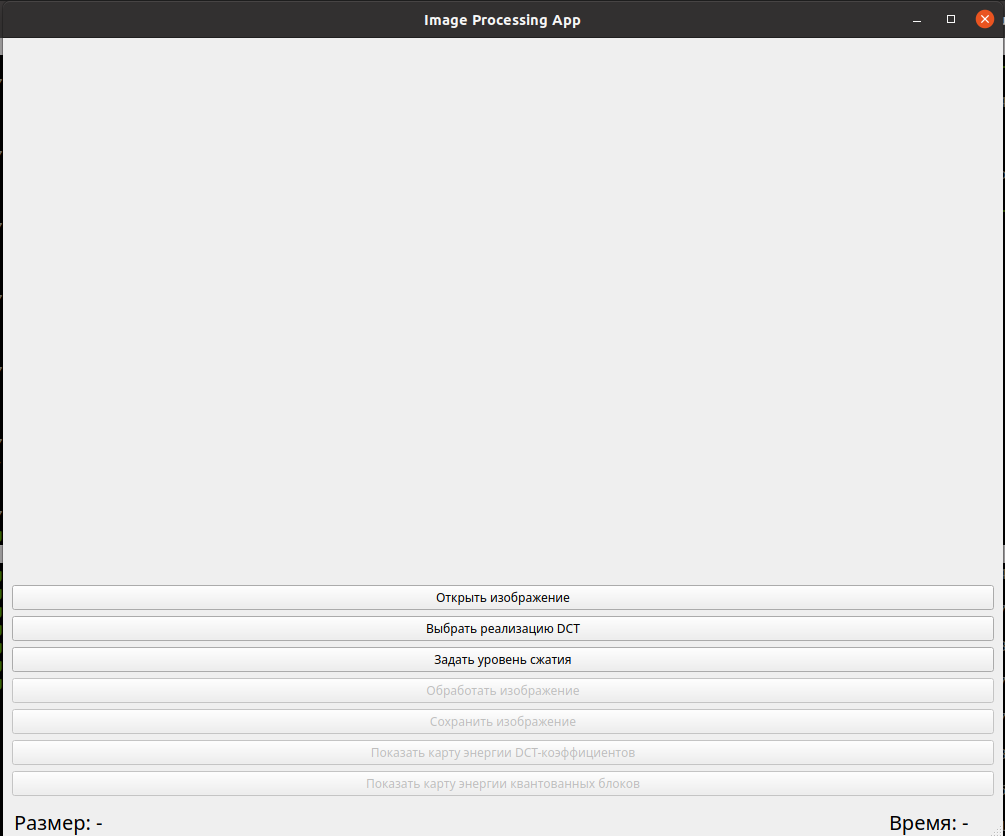
\includegraphics[width=0.7\textwidth]{/home/evgen/Coursework/app/diplom/images/interface.png}
    \caption{Главное окно приложения.}
    \label{fig:interface}
\end{figure}



\subsubsection{Основные элементы интерфейса:}

\begin{itemize}
    \item \textbf{Открыть изображение}

    Позволяет выбрать изображение в формате PNG или JPEG для обработки.
    
    \begin{figure}[h!]
        \centering
        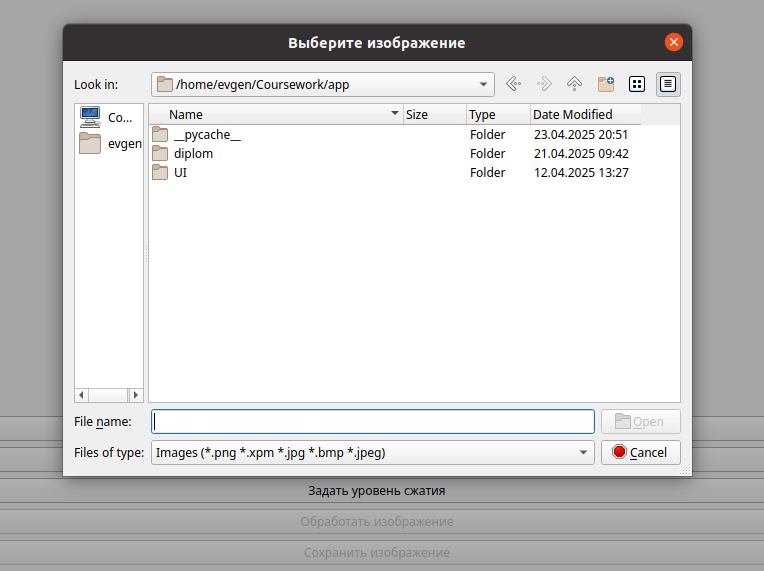
\includegraphics[width=0.5\textwidth]{/home/evgen/Coursework/app/diplom/images/win_choice.png}
        \caption{Окно выбора изображений.}
        \label{fig:win_choice}
    \end{figure}



    \item \textbf{Выбрать реализацию DCT}

    В графическом интерфейсе приложения предусмотрена возможность выбора реализации дискретного косинусного преобразования (DCT). 
    Пользователю предлагаются два варианта:

    Собственная реализация DCT, разработанная вручную в рамках дипломного проекта;
    
    Готовая реализация из библиотеки SciPy (scipy.fftpack.dct), используемая в качестве эталонной и производительной альтернативы.
    
    Это позволяет провести наглядное сравнение корректности и эффективности обеих реализаций, а также удостовериться в соответствии собственной реализации общепринятым стандартам.

    \begin{figure}[h!]
        \centering
        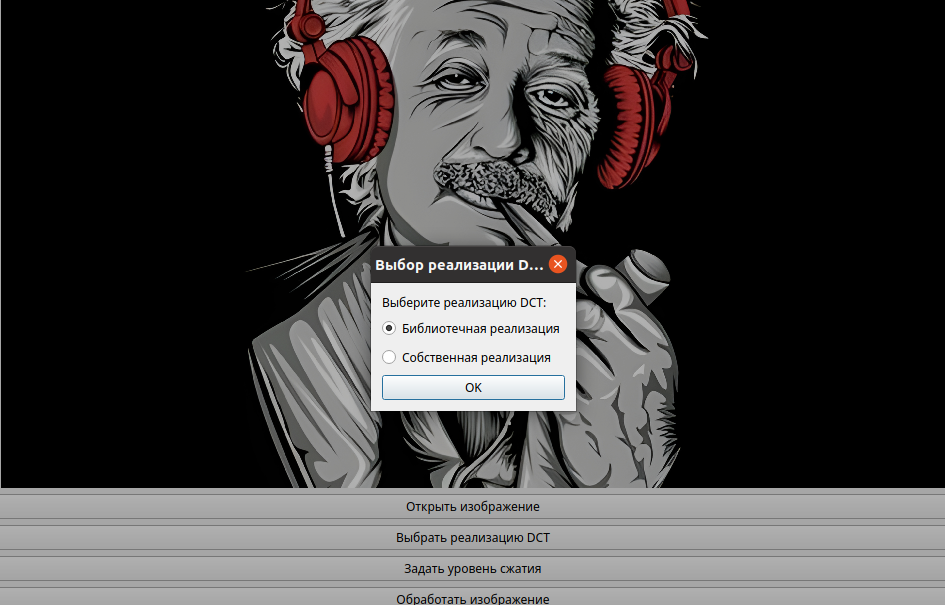
\includegraphics[width=0.8\textwidth]{/home/evgen/Coursework/app/diplom/images/choice_dct.png}
        \caption{Выбрать реализацию DCT.}
        \label{fig:choice_dct}
    \end{figure}



    \item \textbf{Задать уровень сжатия}
    
    Предусмотрена возможность установки уровня сжатия, который напрямую влияет на коэффициенты квантования. 
    Более высокий уровень сжатия приводит к агрессивному округлению высокочастотных коэффициентов, 
    что уменьшает объём выходного файла, но может снизить качество восстановленного изображения. 
    Напротив, меньшие значения сохраняют больше информации, обеспечивая лучшее качество при увеличенном размере файла.

    Это позволяет пользователю находить баланс между качеством изображения и степенью компрессии в зависимости от задач.
    \begin{figure}[h!]
        \centering
        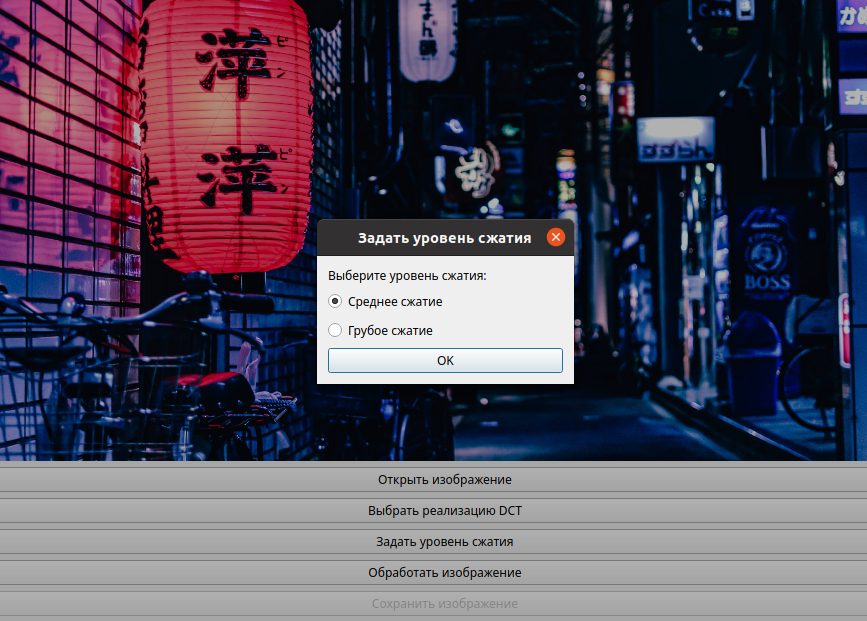
\includegraphics[width=0.9\textwidth]{/home/evgen/Coursework/app/diplom/images/lvl_compres.png}
        \caption{Выбрать уровень сжатия.}
        \label{fig:lvl_compres}
    \end{figure}

    \FloatBarrier

    \item \textbf{Обработать изображение}
    
    После выбора параметров пользователь может запустить процесс обработки, 
    нажав на кнопку \textbf{«Обработать изображение»}. 
    Программа выполняет полный цикл сжатия и восстановления изображения, повторяя основные этапы алгоритма JPEG.

    Сначала изображение преобразуется из цветового пространства RGB в YCbCr.
    Затем изображение разбивается на блоки.
    К каждому блоку применяется дискретное косинусное преобразование (DCT), 
    переводя данные из пространственной области в частотную. 
    Полученные коэффициенты проходят этап квантования, 
    при котором незначительные высокочастотные компоненты подавляются — это и есть основное сжатие с потерями.

    После квантования коэффициенты сканируются по зигзагообразной траектории, что группирует нули, 
    появившиеся в результате округлений. 
    Затем выполняется кодирование методом RLE.

    На финальном этапе происходит декодирование, и вывод получившегося изображения в в окне приложения.

    \begin{figure}[h!]
        \centering
        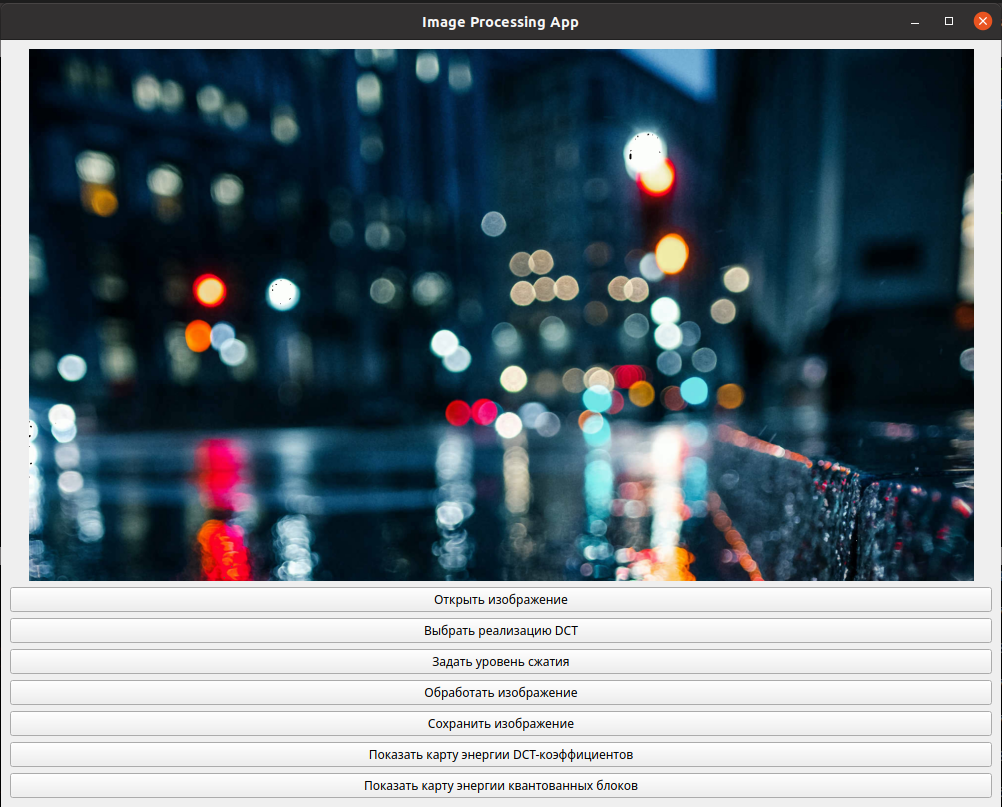
\includegraphics[width=0.9\textwidth]{/home/evgen/Coursework/app/diplom/images/continue.png}
        \caption{Дополнительные элементы.}
        \label{fig:continue}
    \end{figure}


    После завершения обработки становятся доступными дополнительные элементы интерфейса, 
    позволяющие более подробно проанализировать результат.

    \FloatBarrier

    \item \textbf{Сохранить изображение}
    
    Позволяет сохранить на диске восстановленное после сжатия изображение в формате JPEG.

    \begin{figure}[h!]
        \centering
        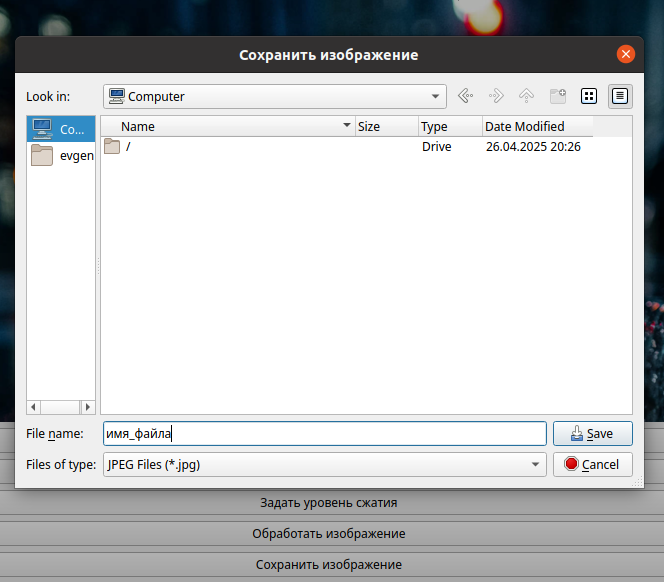
\includegraphics[width=0.9\textwidth]{/home/evgen/Coursework/app/diplom/images/save_img.png}
        \caption{Сохранить изображение.}
        \label{fig:save_img}
    \end{figure}


    \FloatBarrier
    \item \textbf{Показать карту энергии DCT-коэффициентов}
    
    Данный элемент визуализирует вклад различных частотных компонент в изображение до этапа квантования. 
    Это позволяет понять, какие частоты наиболее значимы в передаче визуальной информации


    \begin{figure}[h!]
        \centering
        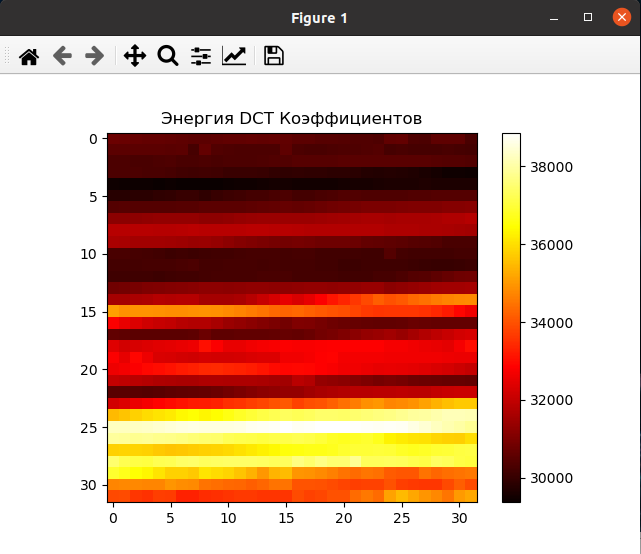
\includegraphics[width=0.9\textwidth]{/home/evgen/Coursework/app/diplom/images/map_energy.png}
        \caption{Карта энергии DCT-коэффициентов.}
        \label{fig:map_energy}
    \end{figure}


    \FloatBarrier

    \item \textbf{Показать карту энергии квантованных блоков} 

    Отображает распределение энергии после квантования. 
    Данная визуализация помогает оценить потери, вызванные округлением коэффициентов.

    \begin{figure}[h!]
        \centering
        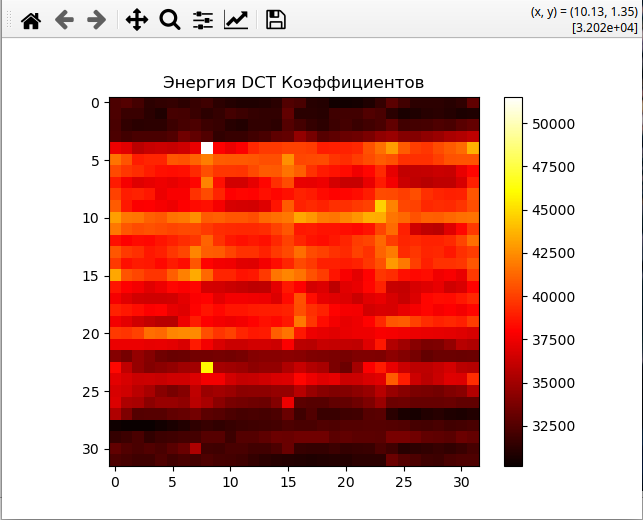
\includegraphics[width=0.9\textwidth]{/home/evgen/Coursework/app/diplom/images/map_quant.png}
        \caption{Карта энергии квантованных блоков.}
        \label{fig:map_quant}
    \end{figure}

\end{itemize}

\FloatBarrier
В нижней части окна приложения отображаются числовые параметры, 
предоставляющие пользователю информацию о производительности и эффективности алгоритма сжатия:
\begin{itemize}
    \item \textbf{Размер изображений} — отображает объём изображения до и после обработки, в килобайтах. 
    Этот позволяет пользователю сравнить исходный размер файла с результатом сжатия и оценить, 
    насколько сильно уменьшился объём данных.

    \item \textbf{Время обработки} — показывает общее время, затраченное на выполнение всех этапов алгоритма, 
    включая преобразование цветового пространства, разбиение на блоки, дискретное косинусное преобразование, 
    квантование, кодирование с помощью RLE и последующее восстановление изображения. 
    Этот показатель даёт представление о производительности реализации и позволяет сравнивать 
    скорость работы разных вариантов DCT или уровней сжатия.
\end{itemize}


\begin{figure}[h!]
    \centering
    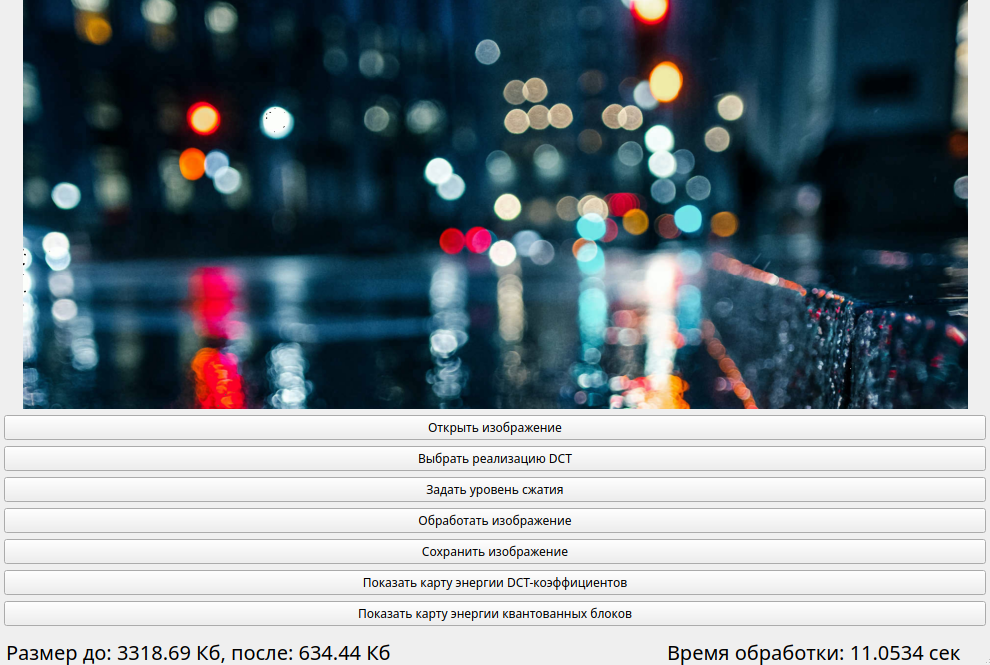
\includegraphics[width=0.9\textwidth]{/home/evgen/Coursework/app/diplom/images/time_size.png}
    \caption{Числовые параметры.}
    \label{fig:time_size}
\end{figure}



\clearpage
\section{Результаты и выводы}


%%%%%%%%%%%%%%%%%%%%%%%%%%%%%%%%%
На рисунке \ref{fig:ssim_vs_quant} представлена зависимость метрики SSIM от уровня квантования. 

SSIM (Structural Similarity Index) — это метрика, используемая для оценки качества изображения, 
которая измеряет, насколько два изображения похожи на уровне их структуры. 
Она была предложена в 2004 году как улучшение для традиционных методов оценки качества изображений, 
таких как PSNR (Peak Signal-to-Noise Ratio). 
SSIM учитывает восприятие человеческим глазом и включает в себя три важнейших аспекта изображения:
\begin{itemize}
    \item Яркость (Luminance) — измеряет разницу в яркости между двумя изображениями.
    \item Контраст (Contrast) — оценивает, насколько изображения различаются по контрасту.
    \item Структура (Structure) — учитывает, насколько хорошо сохраняется структура или текстура изображения, например, линии, края и другие важные детали.
\end{itemize}
(значения ближе к 1 означают высокое качество).

\textbf{Формула SSIM}

Метрика рассчитывается по следующей формуле:
\begin{equation}
\text{SSIM}(x, y) = 
\frac{(2\mu_x\mu_y + C_1)(2\sigma_{xy} + C_2)}
     {(\mu_x^2 + \mu_y^2 + C_1)(\sigma_x^2 + \sigma_y^2 + C_2)}
\end{equation}


\begin{itemize}
    \item $x, y$ — сравниваемые изображения (или блоки изображений).
    \item $\mu_x$ — среднее значение яркости изображения $x$:
    \[
        \mu_x = \frac{1}{N} \sum_{i=1}^{N} x_i
    \]
    \item $\mu_y$ — среднее значение яркости изображения $y$.
    
    \item $\sigma_x^2$ — дисперсия яркости изображения $x$:
    \[
        \sigma_x^2 = \frac{1}{N-1} \sum_{i=1}^{N} (x_i - \mu_x)^2
    \]
    \item $\sigma_y^2$ — дисперсия яркости изображения $y$.
    
    \item $\sigma_{xy}$ — ковариация между $x$ и $y$:
    \[
        \sigma_{xy} = \frac{1}{N-1} \sum_{i=1}^{N} (x_i - \mu_x)(y_i - \mu_y)
    \]
    
    \item $C_1 = (K_1 L)^2$, $C_2 = (K_2 L)^2$ — стабилизирующие константы:
    \begin{itemize}
        \item $L$ — динамический диапазон значений пикселей (например, 255 для 8-битных изображений),
        \item $K_1 = 0.01$, $K_2 = 0.03$.
    \end{itemize}
\end{itemize}



\begin{figure}[H]
    \centering
    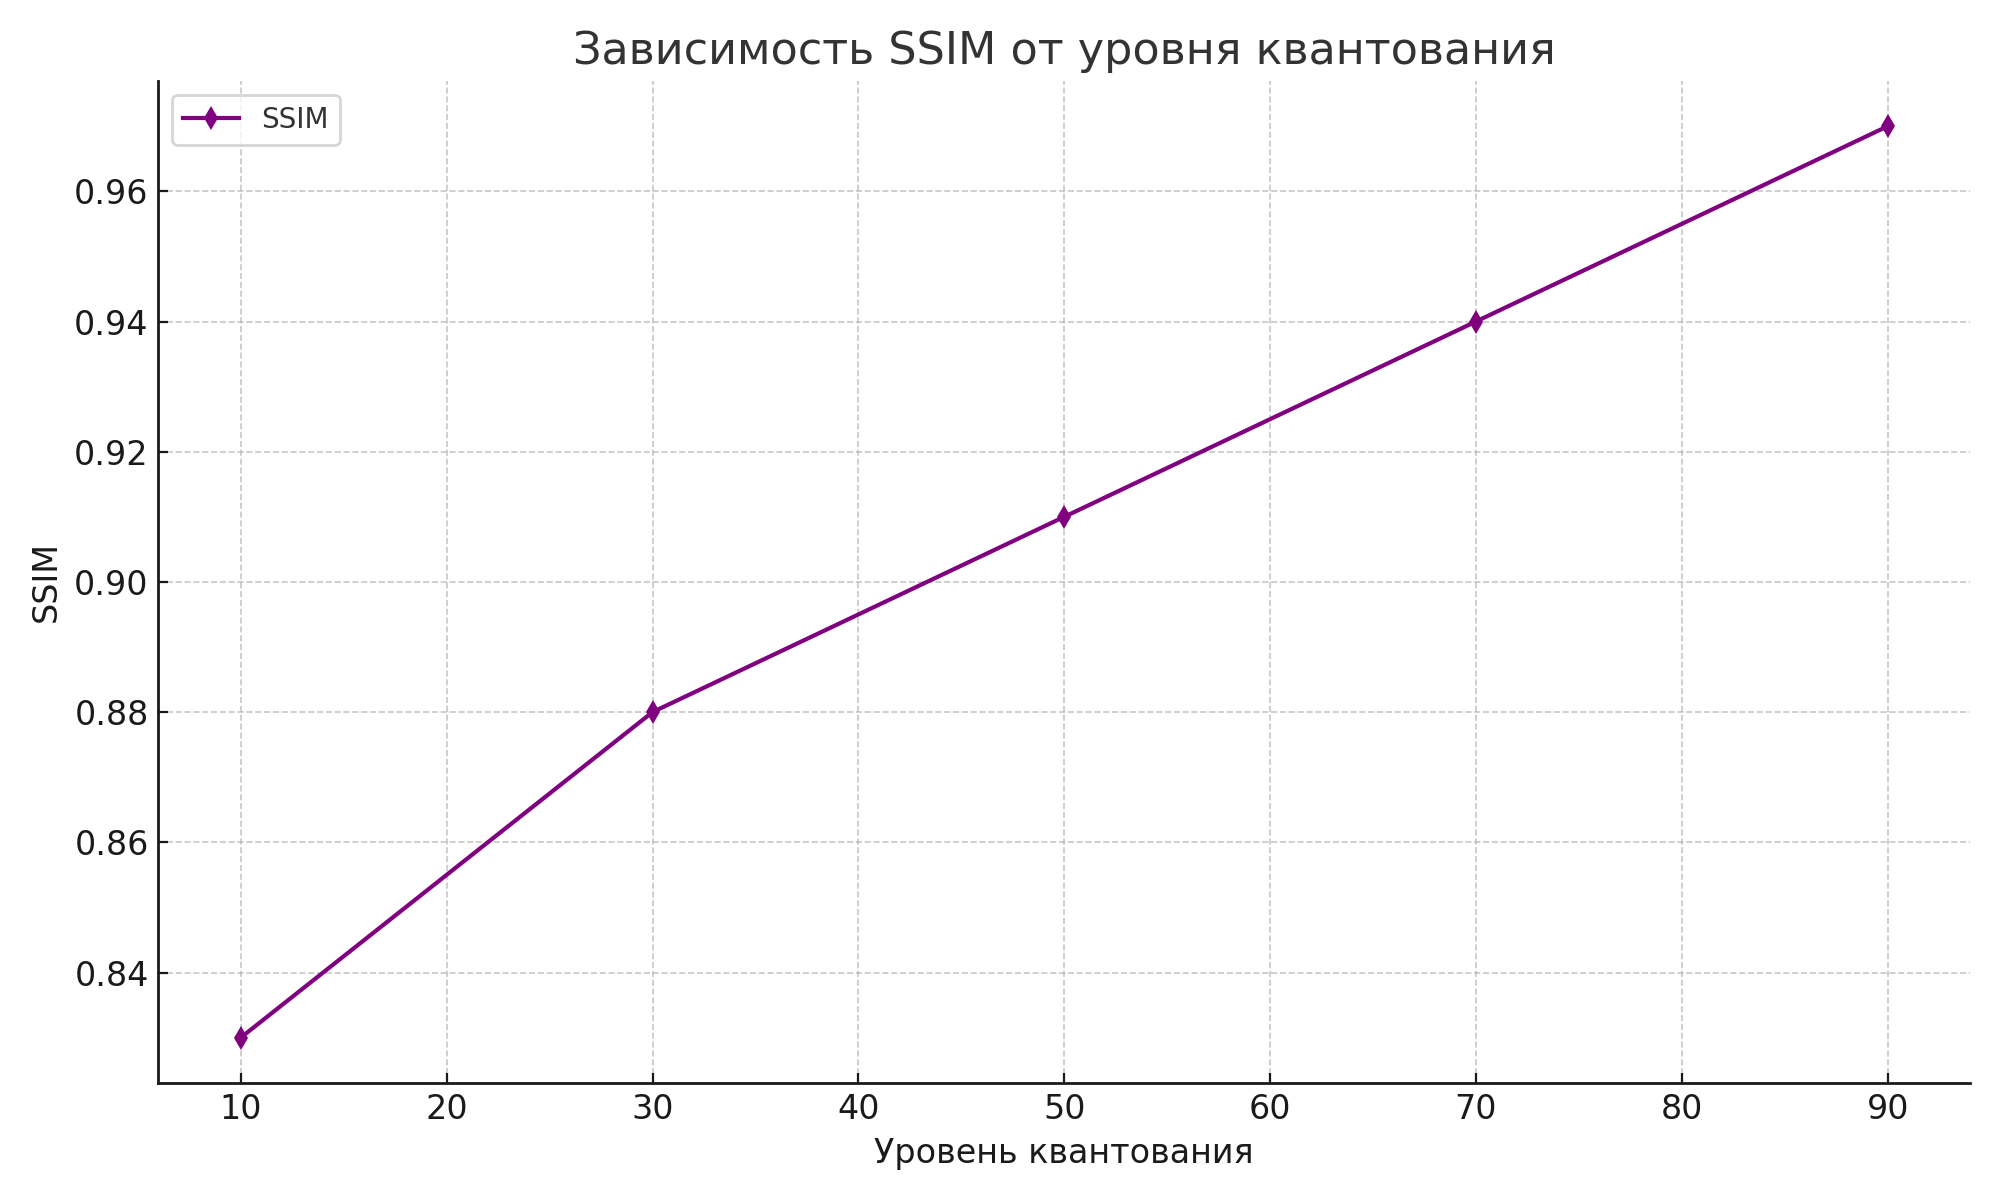
\includegraphics[width=0.9\textwidth]{/home/evgen/Coursework/app/diplom/images/ssim_vs_quant.png}
    \caption{Зависимость метрики SSIM от уровня квантования.}
    \label{fig:ssim_vs_quant}
\end{figure}

График показывает, что при увеличении уровня квантования 
(то есть более агрессивном удалении высокочастотной информации) метрика SSIM уменьшается. 
Это соответствует ожиданиям: чем сильнее сжатие, тем больше потерь информации и ниже визуальное качество. 
На небольших уровнях квантования (до, 70\%) качество остаётся почти неизменным, но при уровнях выше 70\% наблюдается значительное ухудшение. 
Это даёт возможность выбрать компромисс между степенью сжатия и визуальным качеством.


%%%%%%%
\clearpage
На рисунке \ref{fig:psnr_vs_blocksize} показано, как изменяется метрика PSNR (Peak Signal-to-Noise Ratio) в зависимости от размера блока, 
используемого для дискретного косинусного преобразования.

\begin{figure}[H]
    \centering
    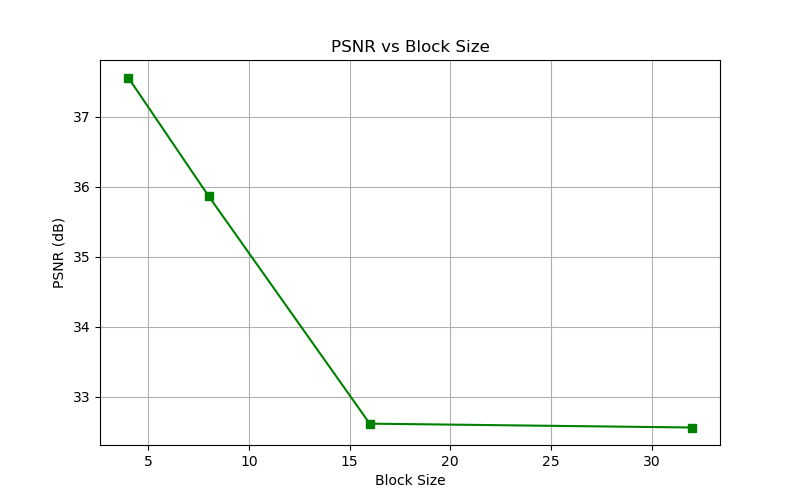
\includegraphics[width=1\textwidth]{/home/evgen/Coursework/app/diplom/images/psnr_vs_block_size.png}
    \caption{Зависимость PSNR от размера блока.}
    \label{fig:psnr_vs_blocksize}
\end{figure}

PSNR — это классическая метрика оценки искажения сигнала (в данном случае, изображения); 
более высокие значения указывают на лучшее качество восстановления. При небольшом размере блока 
(8×8) значения PSNR максимальны, что объясняется более точной локальной аппроксимацией содержимого. 
С увеличением размера блока (например, 32×32) точность снижается из-за усреднения на более крупных 
участках изображения, что приводит к потере деталей и снижению PSNR.

\begin{equation}
\text{PSNR} = 10 \cdot \log_{10} \left( \frac{MAX_I^2}{\text{MSE}} \right)
\end{equation}


\begin{itemize}
    \item $MAX_I$ — максимальное значение интенсивности пикселя (обычно 255).
    \item $\text{MSE}$ — среднеквадратичная ошибка между оригинальным и восстановленным изображениями:
    \[
    \text{MSE} = \frac{1}{MN} \sum_{i=1}^{M} \sum_{j=1}^{N} \left[ I(i,j) - K(i,j) \right]^2
    \]
    \item $I(i,j)$ — значение пикселя в оригинальном изображении.
    \item $K(i,j)$ — значение пикселя в искажённом изображении.
\end{itemize}



Таким образом, блоки 8×8 являются оптимальными с точки зрения компромисса между сжатием и качеством, 
что подтверждает выбор JPEG-стандарта.

%%%%
Рисунок \ref{fig:ssim_vs_blocksize} демонстрирует, как изменяется метрика SSIM в зависимости от размера блока. 
Аналогично PSNR, максимальное качество достигается при использовании размера 4×4, однако для сохранения скорости обработки
компромиссом является размер $8 \times 8$. 
По мере увеличения блока падает точность локального анализа изображения, 
что особенно критично для SSIM — метрики, учитывающей локальные структуры и контраст.

\begin{figure}[H]
    \centering
    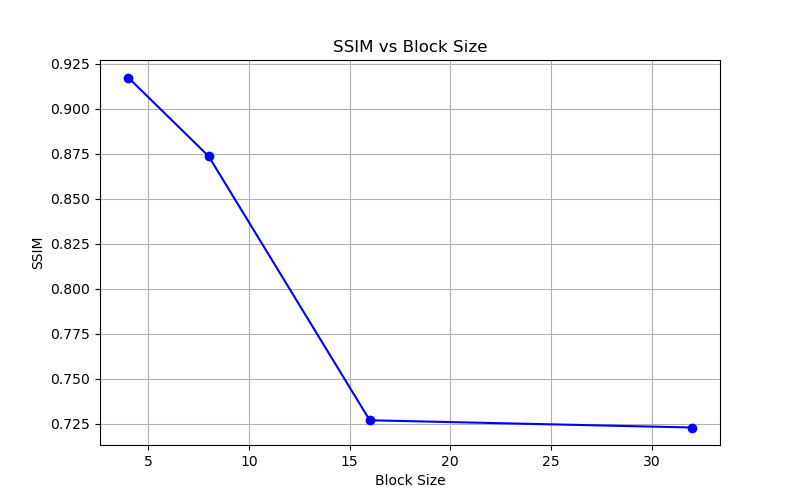
\includegraphics[width=1\textwidth]{/home/evgen/Coursework/app/diplom/images/ssim_vs_block_size.png}
    \caption{Зависимость SSIM от размера блока.}
    \label{fig:ssim_vs_blocksize}
\end{figure}

Таким образом, большие блоки ухудшают восприятие изображения, особенно в областях с высокой детализацией. 
Это подчёркивает важность выбора разумного размера блока для сохранения визуального качества при сжатии.


%%%%%
На рисунке \ref{fig:time_vs_blocksize} представлена зависимость времени обработки изображения от размера блока. 
Время измерялось в миллисекундах для полного цикла сжатия и восстановления изображения фиксированного 
размера (например, 512×512 пикселей).

\begin{figure}[H]
    \centering
    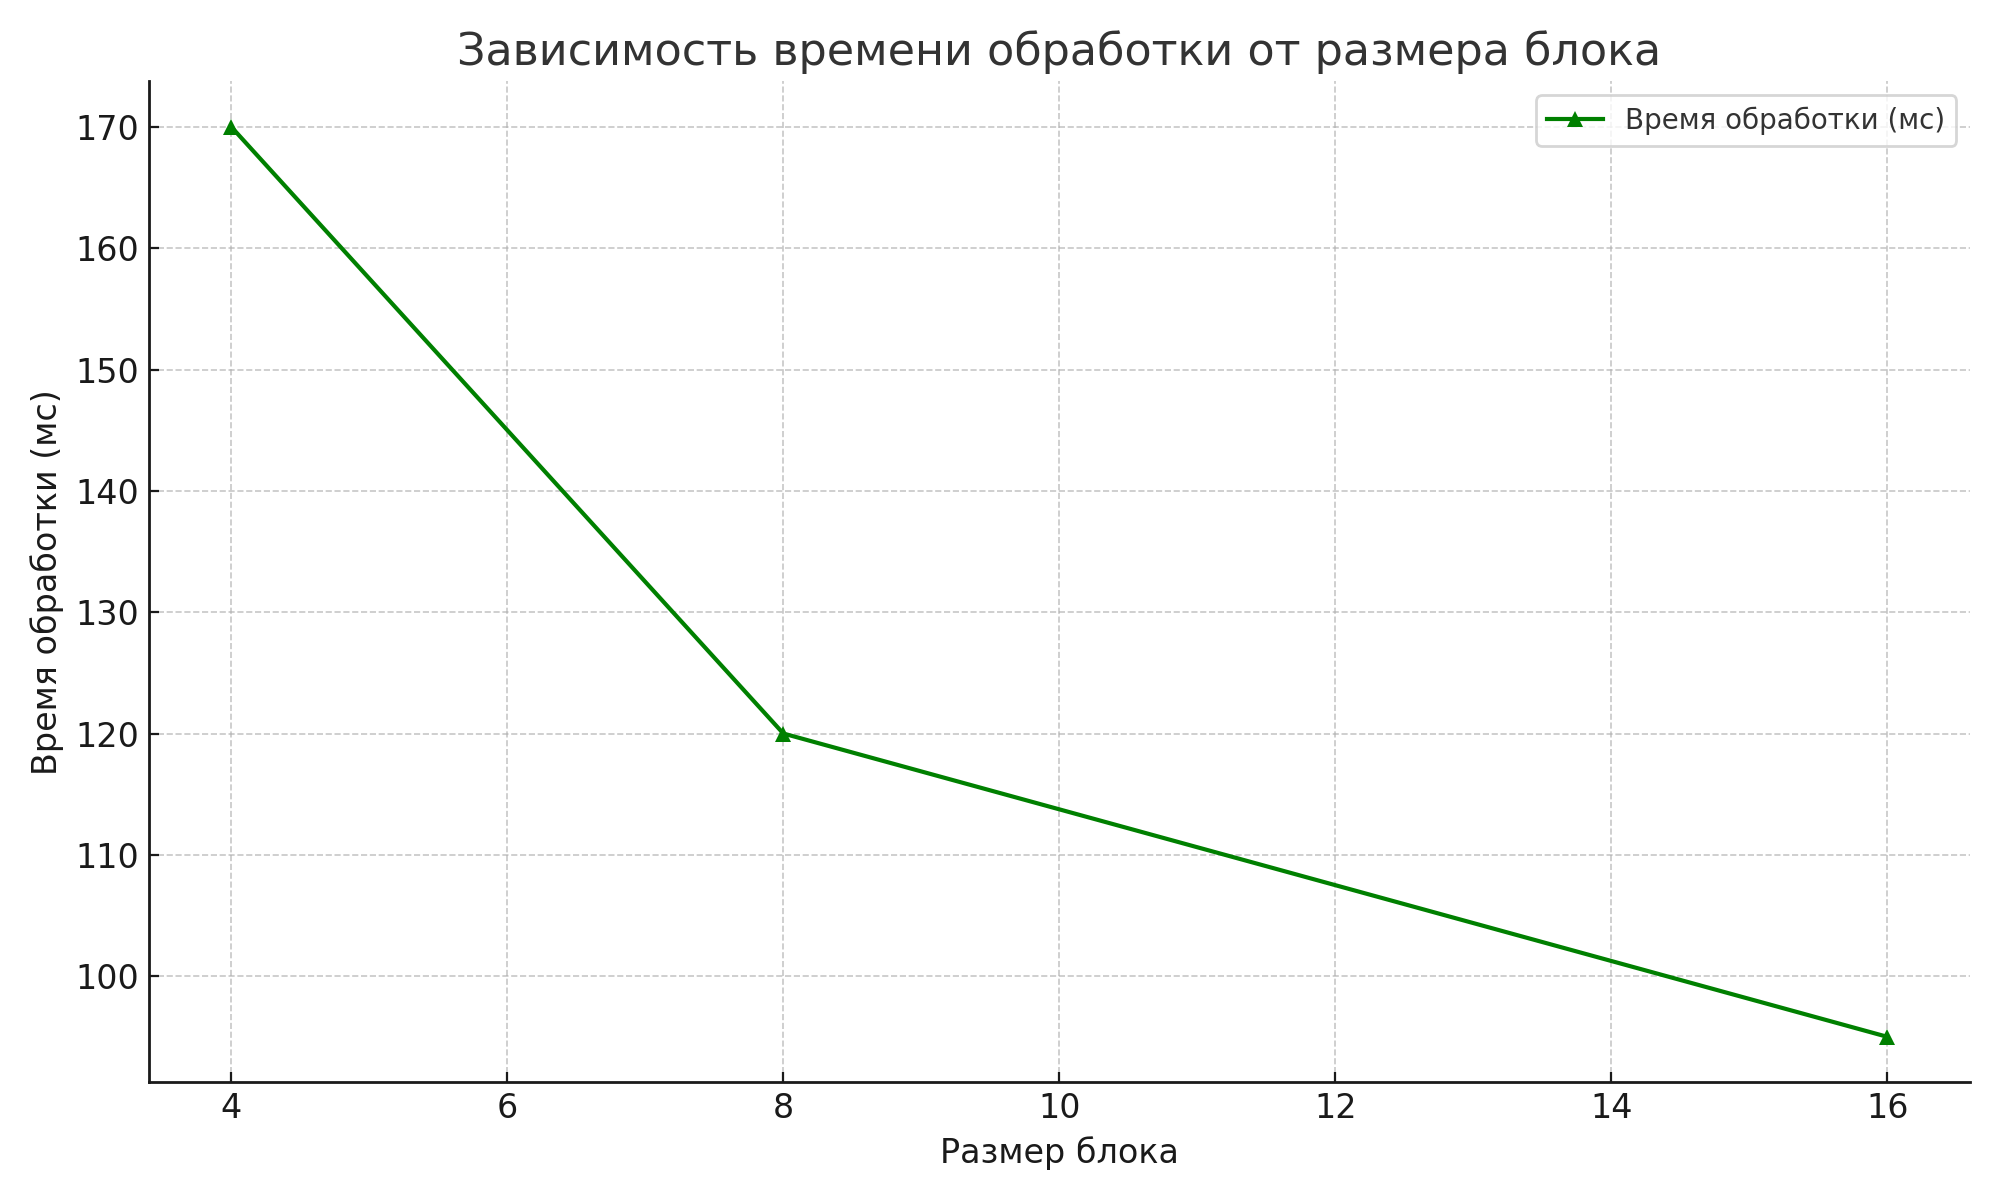
\includegraphics[width=0.9\textwidth]{/home/evgen/Coursework/app/diplom/images/time_vs_blocksize.png}
    \caption{Зависимость времени обработки от размера блока.}
    \label{fig:time_vs_blocksize}
\end{figure}

График показывает, что с увеличением размера блока общее количество блоков уменьшается, 
что снижает число вычислений (например, DCT и RLE выполняются реже), и, как следствие, 
сокращается общее время обработки. 
Однако при слишком больших блоках может наблюдаться незначительный рост времени из-за увеличения объёма 
обработки каждого отдельного блока и возможного падения эффективности кэширования.

Этот график полезен для анализа производительности и помогает выбрать подходящий размер блока в 
зависимости от требований к скорости и качеству.



%%%%%%%%%%%%%%%%%%%%%
\subsubsection{Влияние квантования на цветовые искажения}

В процессе экспериментов было замечено, что неправильно подобранные коэффициенты квантования особенно для 
цветовых компонент (Cb и Cr) могут вызывать искажения цветовой палитры изображения.

На ряде примеров наблюдалось:

\begin{itemize}
    \item Уход цвета в сторону сине-зелёных или красных оттенков;
    \item Появление "грязных" артефактов в областях с однородным цветом;
    \item Потеря цветовой согласованности на границах объектов.
\end{itemize}


\begin{figure}[H]
    \centering
    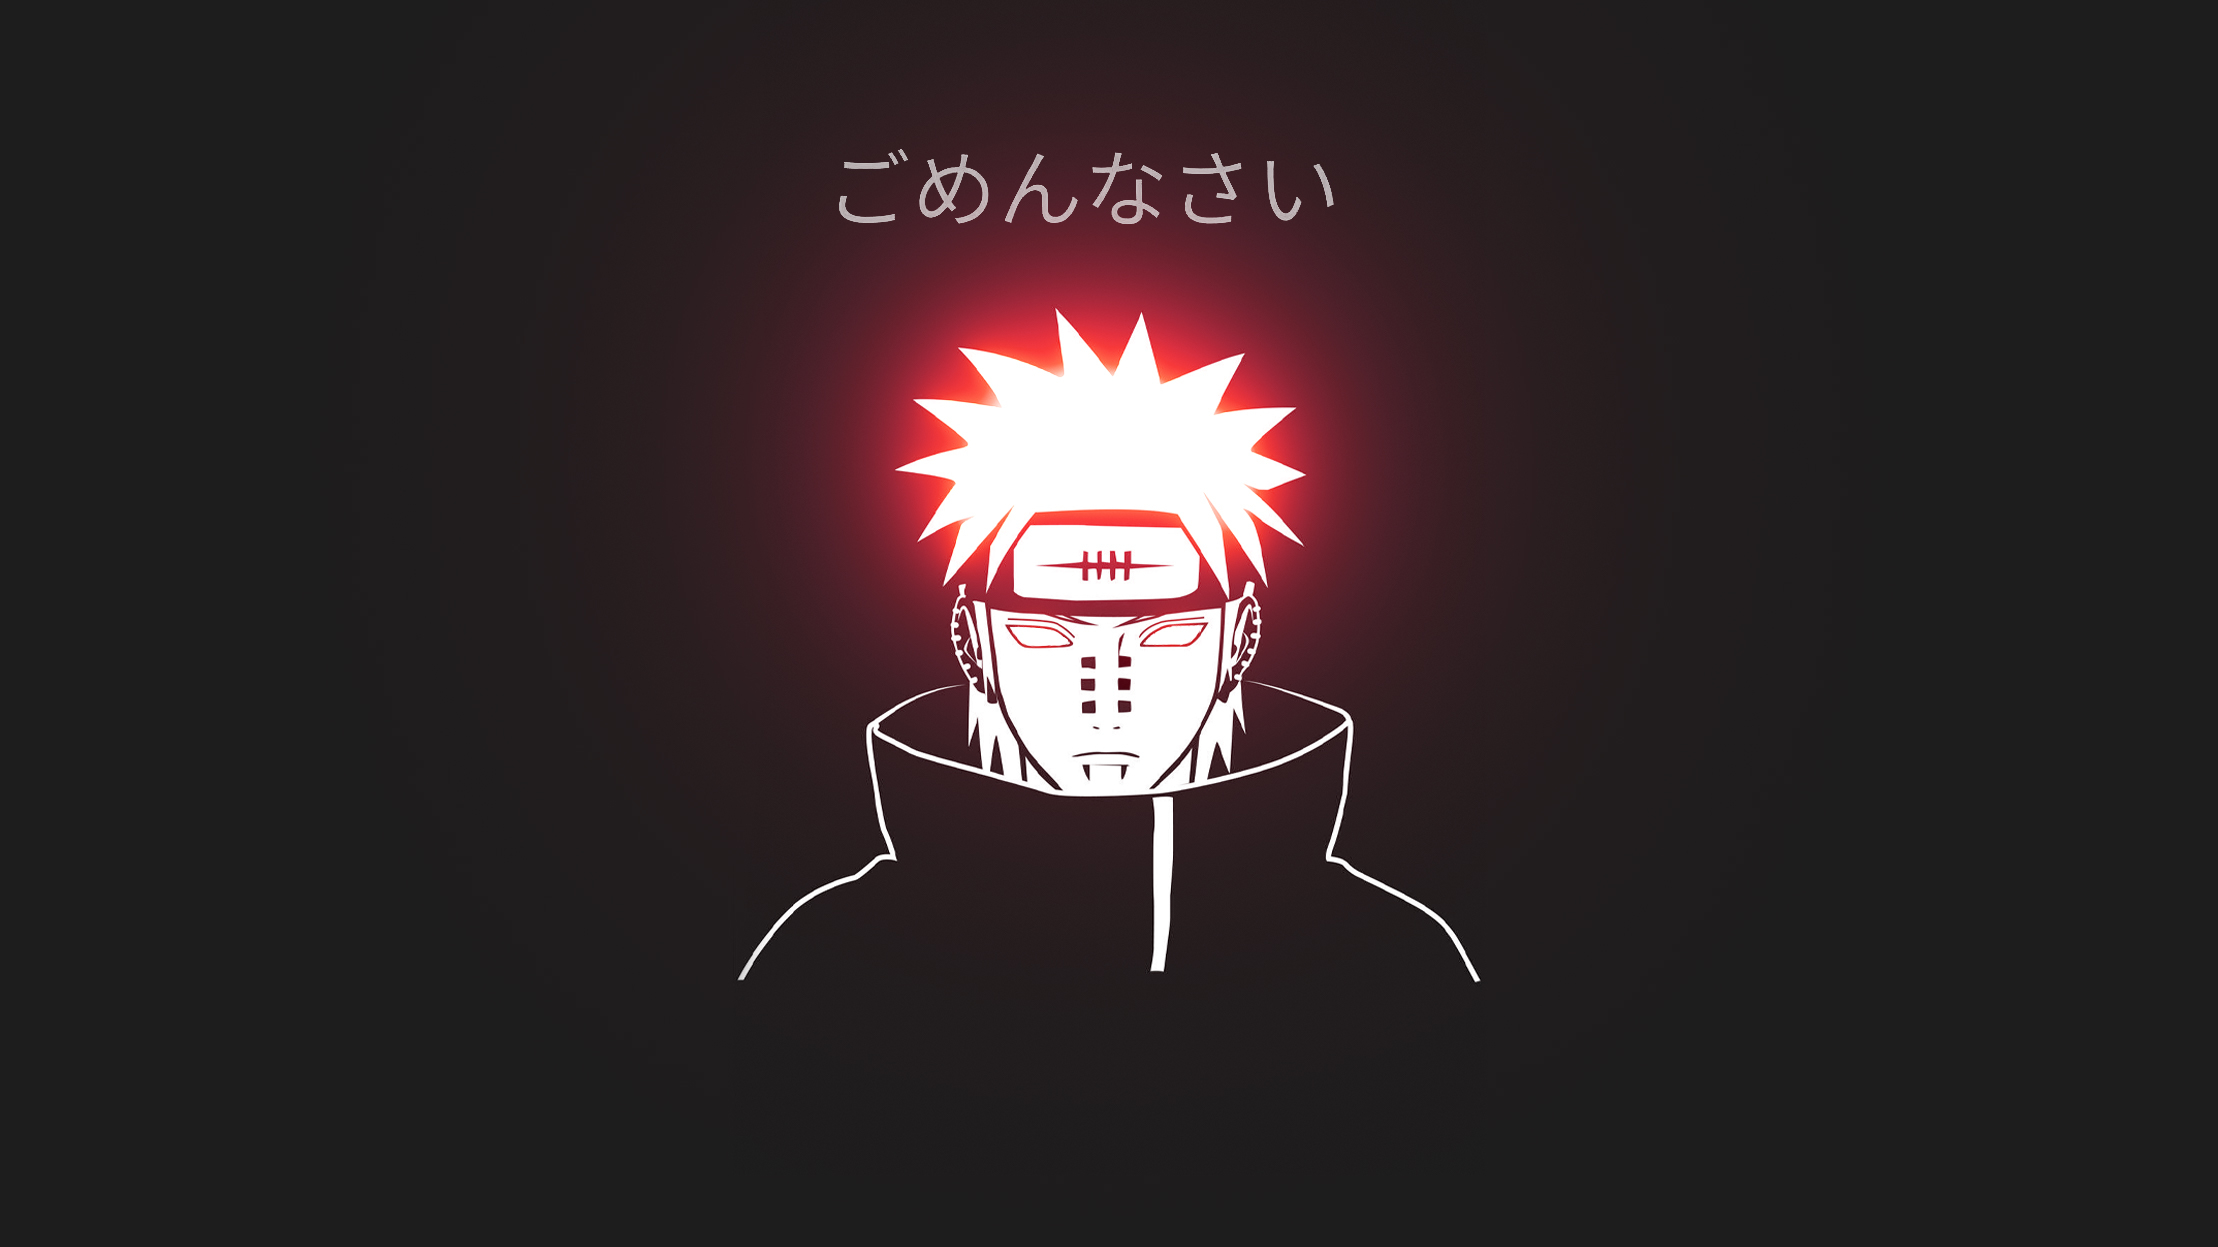
\includegraphics[width=0.9\textwidth]{/home/evgen/Coursework/app/diplom/images/base_image.jpg}
    \caption{До квантования с неправильно подобранными коэффициентами.}
    \label{fig:base_image}
\end{figure}

 
\begin{figure}[H]
    \centering
    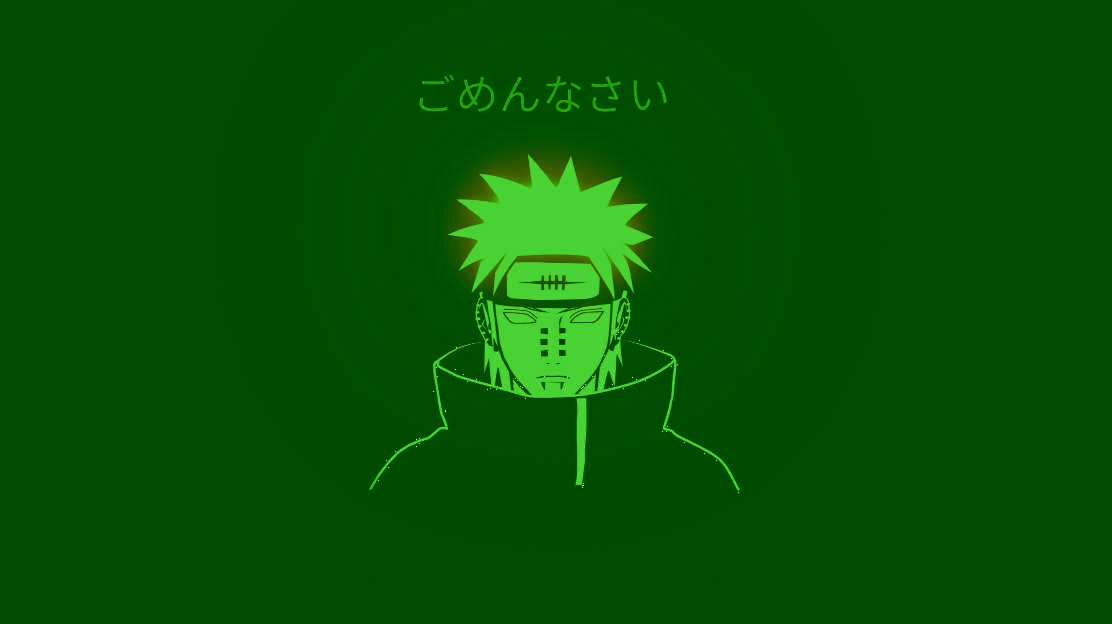
\includegraphics[width=0.9\textwidth]{/home/evgen/Coursework/app/diplom/images/change_color1.jpg}
    \caption{После квантования с неправильно подобранными коэффициентами.}
    \label{fig:change_color}
\end{figure}

На рисунке \ref{fig:change_color} видно, как цветовая палитра сместилась в сторону зеленого цвета.

Это подчёркивает важность отдельного подбора квантования для яркостного и цветовых каналов, 
что в классическом JPEG также учитывается.


%%%%%%%%%%%%%%%%%%%%%%
\subsubsection{Проявление артефактов}
Но степень квантования и неправильно подобрнанные коэффициенты для матриц квантования не единственные причины
из-за которых могут появиться артефакты в области границ или неоднородного цвета.

При использовании блоков большого размера (например, $32 \times 32$), 
на изображениях начали проявляться артефакты в виде белых точек или резких границ между блоками.

Особенности:
\begin{itemize}
    \item Артефакты особенно видны в текстурированных или теневых областях.
    \item В некоторых случаях они проявляются как “решётка” из блоков, так называемый "блокинг-эффект".
    \item В наиболее заметных случаях артефакты выглядят как одиночные белые пиксели, особенно на тёмных участках изображения.
\end{itemize}


\begin{figure}[H]
    \centering
    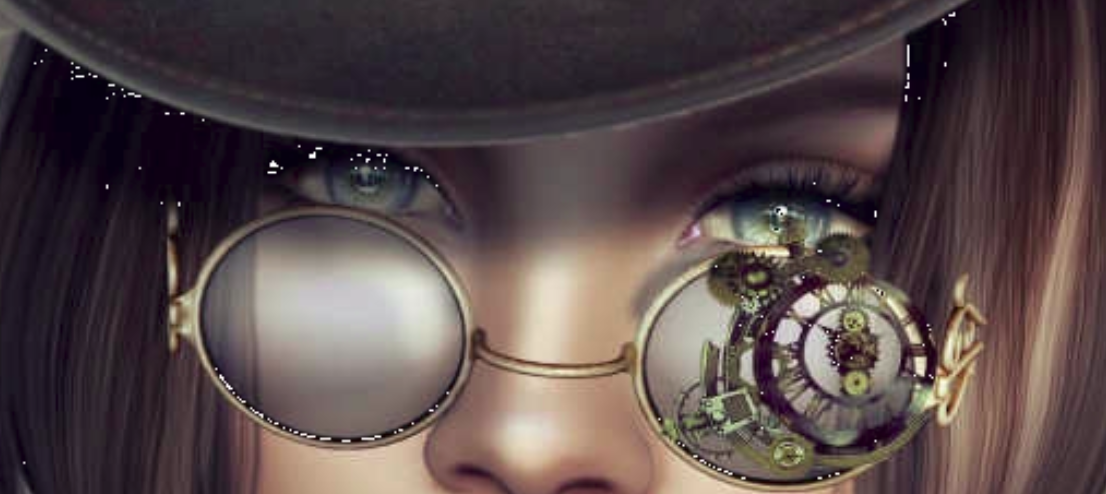
\includegraphics[width=0.9\textwidth]{/home/evgen/Coursework/app/diplom/images/artefacts_white_pixel.png}
    \caption{Артефакты в виде белых пикселей.}
    \label{fig:artefacts_white_pixel}
\end{figure}

 Дополнительную нагрузку на алгоритм создаёт избыточная детализация — большое количество текстур, 
 тонких линий и резких переходов в изображении ухудшают результаты аппроксимации в частотной области. 
 Особенно чувствительными к искажениям оказываются области с высокими градиентами цвета, 
 где даже при умеренном сжатии возможно появление визуальных дефектов. 
 Таким образом, причины появления артефактов комплексны и зависят как от параметров алгоритма, 
 так и от характера самого изображения.


%%%%%%%%%%%%%%%%%%%%%%%%%%%
\subsubsection{Способы устранения визуалных дефектов}

На основе экспериментов были выделены практические приёмы снижения артефактов:

\begin{enumerate}
    \item \textbf{Снижение уровня квантования}
    Уменьшает потери, особенно в чувствительных областях изображения (тени, переходы, кожа и т.п.).

    \item \textbf{Раздельное квантование Y и Cb/Cr}
    Позволяет сохранять цветовую палитру более точно, снижая искажения. Так же удобно, для анализа отдельных
    компонентов, упрощает посиск ошибок в приложении и его отладку.

    \item \textbf{Уменьшение размера блока (например, до 4×4)}
    Повышает точность локального анализа, особенно в участках с деталями и границами.
    Однако может значительно увеличить время обработки изображения. В этом случае можно двигаться в сторону 
    параллелизма и модификации дискретного косинусного преобразования (DCT) для ускорения.

    \item \textbf{Подбор и адаптация матриц квантования}
    Более мягкие матрицы снижают потери на высоких частотах и уменьшают риск появления "белых точек".

    \item \textbf{Пред/пост обработка изображения (например, фильтрация шума)}
    Уменьшение шумов до сжатия помогает избежать ненужных артефактов. После сжатия, так же можно применять
    фильтры для устранения уже имеющегося шума.

    \item \textbf{Адаптация к содержимому}
    Возможность выбора параметров сжатия в зависимости от анализа изображения 
    (например, в сложных участках использовать более мелкие блоки и меньшую степень квантования).
    Или разработать тест 
\end{enumerate}
